\documentclass{article}

\usepackage{a4}
\usepackage{amsmath}
\usepackage{amssymb}
\usepackage{ctex}
\usepackage{booktabs}
\usepackage{graphicx}
\usepackage{subfigure}
\usepackage{subcaption}
\usepackage{float}
\usepackage{hyperref}
\usepackage{xurl}
\usepackage{enumitem}
\usepackage{array}
\usepackage{longtable}
\usepackage{multirow}
\usepackage{fvextra}

\hypersetup{colorlinks=true,linkcolor=black,urlcolor=blue,citecolor=black}
\setlist[itemize]{nosep,leftmargin=1.8em}
\setlist[enumerate]{nosep,leftmargin=1.8em}
\captionsetup{font=small}
\setlength{\emergencystretch}{3em}
\renewcommand{\arraystretch}{1.2}
\RecustomVerbatimEnvironment{verbatim}{Verbatim}{
  breaklines=true,
  breakanywhere=true,
  fontsize=\small
}
\newcommand{\sourcecode}[2]{
  \subsubsection*{#1}
  \noindent 对应文件：\path{#2}
  \VerbatimInput[
    breaklines=true,
    breakanywhere=true,
    fontsize=\small
  ]{#2}
}

\title{计算机组成原理 Project1 实验报告（Week 3）\\8位定点卷积--激活--池化链运算器设计}
\author{鲁昕宁 2414015}
\date{\today}

\begin{document}

\maketitle
\begin{center}
  \url{https://github.com/SidneyLu/Computer-Organization-and-Design-NKU-CS/tree/master/project1}
\end{center}

\newpage

\section{优化模块设计}
本部分详细介绍优化模块的设计与验证。

\subsection{优化模块源码}
在基础模块之上，实现了以下优化模块：

\sourcecode{模块 \texttt{mul8\_booth\_wallace} 的 Verilog 源码}{../src/optimized/mul8_booth_wallace.v}
\sourcecode{模块 \texttt{simd\_add8x4} 的 Verilog 源码}{../src/optimized/simd_add8x4.v}
\sourcecode{模块 \texttt{simd\_mul8x4} 的 Verilog 源码}{../src/optimized/simd_mul8x4.v}
\sourcecode{模块 \texttt{simd\_relu8x4} 的 Verilog 源码}{../src/optimized/simd_relu8x4.v}
\sourcecode{模块 \texttt{simd\_avgpool2x2\_8bit} 的 Verilog 源码}{../src/optimized/simd_avgpool2x2_8bit.v}
\sourcecode{模块 \texttt{mul8\_dsp48e1} 的 Verilog 源码}{../src/optimized/mul8_dsp48e1.v}
\sourcecode{模块 \texttt{simd\_mul8x4\_dsp} 的 Verilog 源码}{../src/optimized/simd_mul8x4_dsp.v}

优化版本顶层模块源码如下：

\sourcecode{顶层 \texttt{cnn\_compare\_booth\_top} 的 Verilog 源码}{../src/optimized/cnn_compare_booth_top.v}
\sourcecode{顶层 \texttt{cnn\_compare\_booth\_simd\_top} 的 Verilog 源码}{../src/optimized/cnn_compare_booth_simd_top.v}
\sourcecode{顶层 \texttt{cnn\_compare\_booth\_simd\_pipe\_top} 的 Verilog 源码}{../src/optimized/cnn_compare_booth_simd_pipe_top.v}
\sourcecode{顶层 \texttt{cnn\_compare\_booth\_simd\_pipe\_dsp\_top} 的 Verilog 源码}{../src/optimized/cnn_compare_booth_simd_pipe_dsp_top.v}
\sourcecode{模块 \texttt{cnn\_chain\_core\_booth\_simd} 的 Verilog 源码}{../src/optimized/cnn_chain_core_booth_simd.v}
\sourcecode{模块 \texttt{cnn\_chain\_core\_booth\_simd\_pipe} 的 Verilog 源码}{../src/optimized/cnn_chain_core_booth_simd_pipe.v}
\sourcecode{模块 \texttt{cnn\_chain\_core\_booth\_simd\_pipe\_dsp} 的 Verilog 源码}{../src/optimized/cnn_chain_core_booth_simd_pipe_dsp.v}
\sourcecode{共享卷积核心 \texttt{cnn\_conv3x3\_simd\_core} 的 Verilog 源码}{../src/optimized/cnn_conv3x3_simd_core.v}

\subsection{优化模块仿真}
优化模块的 testbench 覆盖范围如表 \ref{tab:tb-optimized} 所示。

\begin{table}[H]
\centering
\caption{优化模块 testbench}
\label{tab:tb-optimized}
\begin{tabular}{lll}
\toprule
testbench & 验证对象 & 覆盖方式 \\
\midrule
\texttt{tb\_mul\_compare} & BoothWallace 乘法器 & 与 \texttt{mul8} 做 65536 组穷举一致性对比 \\
\texttt{tb\_simd\_mul\_compare} & SIMD / DSP 乘法器 & lane 等价性、边界值与混合模式对比 \\
\bottomrule
\end{tabular}
\end{table}

Vivado 日志显示上述 testbench 均通过：
\begin{itemize}
  \item \texttt{mul8 vs booth/wallace: PASS}
  \item \texttt{tb\_simd\_mul\_compare PASS}
\end{itemize}

\sourcecode{testbench \texttt{tb\_mul\_compare} 的 Verilog 源码}{../sim/tb_mul_compare.v}
\sourcecode{testbench \texttt{tb\_simd\_mul\_compare} 的 Verilog 源码}{../sim/tb_simd_mul_compare.v}

\section{里程碑3：优化与 Vivado 性能验证}
\subsection{综合设置}
综合脚本 \texttt{scripts/run\_vivado\_multi\_synth.tcl} 会依次对以下 5 个顶层执行 \texttt{synth\_design}：
\begin{itemize}
  \item \texttt{cnn\_compare\_base\_top}
  \item \texttt{cnn\_compare\_booth\_top}
  \item \texttt{cnn\_compare\_booth\_simd\_top}
  \item \texttt{cnn\_compare\_booth\_simd\_pipe\_top}
  \item \texttt{cnn\_compare\_booth\_simd\_pipe\_dsp\_top}
\end{itemize}

所有数据均来自 Vivado 2025.1 \texttt{utilization\_report} 与 \texttt{timing\_summary\_report}。

由于本报告在 5ns 约束下比较不同 RTL 结构，因此将估算最小时钟周期写为
\[
T_{\min} \approx 5.000 - \mathrm{WNS}
\]
再用
\[
f_{\max} \approx \frac{1000}{T_{\min}}
\]
估算最高工作频率，用于横向比较不同结构。

\subsection{主四组资源与时序对比}
主对比表仅统计前 4 组，不包含 DSP 替换版。结果如表 \ref{tab:main-compare} 所示。

\begin{table}[H]
\centering
\small
\caption{主四组实验的资源与时序对比}
\label{tab:main-compare}
\begin{tabular}{lrrrrrr}
\toprule
实验组 & LUT & FF & DSP & WNS/ns & 估算$f_{\max}$/MHz & 周期数 \\
\midrule
串行 & 550 & 304 & 0 & -5.546 & 94.82 & 96 \\
串行 + BoothWallace & 532 & 304 & 0 & -5.883 & 91.89 & 96 \\
BoothWallace + SIMD & 8095 & 33 & 0 & -6.030 & 90.66 & 1 \\
BoothWallace + SIMD + 流水线 & 8097 & 287 & 0 & -1.625 & 150.94 & 3 \\
\bottomrule
\end{tabular}
\end{table}

结合表 \ref{tab:main-compare} 与时序报告，可得到以下结论：
\begin{itemize}
  \item 第 2 组在串行框架中将 LUT 从 550 降到 532，但 WNS 从 -5.546\,ns 变为 -5.883\,ns，说明当前关键路径仍主要受串行卷积累加与布线影响，而不是单纯由乘法器级数决定；
  \item 第 3 组将计算周期压缩到 1 个周期，但由于卷积、激活和池化几乎全部落在同一条组合路径上，输入端口到输出寄存器的路径最长，WNS 反而最差；
  \item 第 4 组加入真实三级流水后，WNS 明显改善到 -1.625\,ns，估算最高频率提升到 150.94\,MHz，是主四组中时钟能力最强的实现；
  \item 若按估算频率折算单次计算时延，则第 1/2/3/4 组约为 1012.44\,ns、1044.73\,ns、11.03\,ns 和 19.88\,ns。也就是说，第 3 组在当前结构下具有更短的单次结果延迟，而第 4 组则以更好的时钟能力和更规则的吞吐结构取胜。
\end{itemize}

\begin{figure}[H]
  \centering
  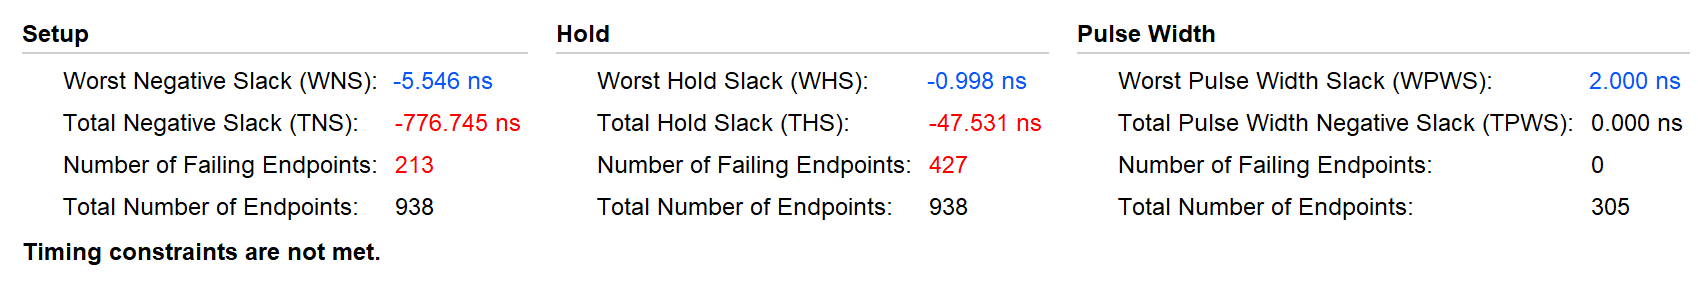
\includegraphics[width=\textwidth]{figures/time1.png}
  \caption{第一组实验的时序报告}
  \label{fig:time1}
\end{figure}
\begin{figure}[H]
  \centering
  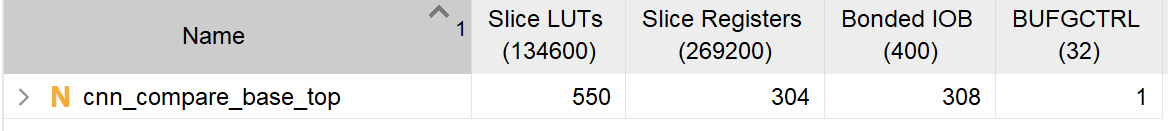
\includegraphics[width=\textwidth]{figures/util1.png}
  \caption{第一组实验的综合报告}
  \label{fig:util1}
\end{figure}

\begin{figure}[H]
  \centering
  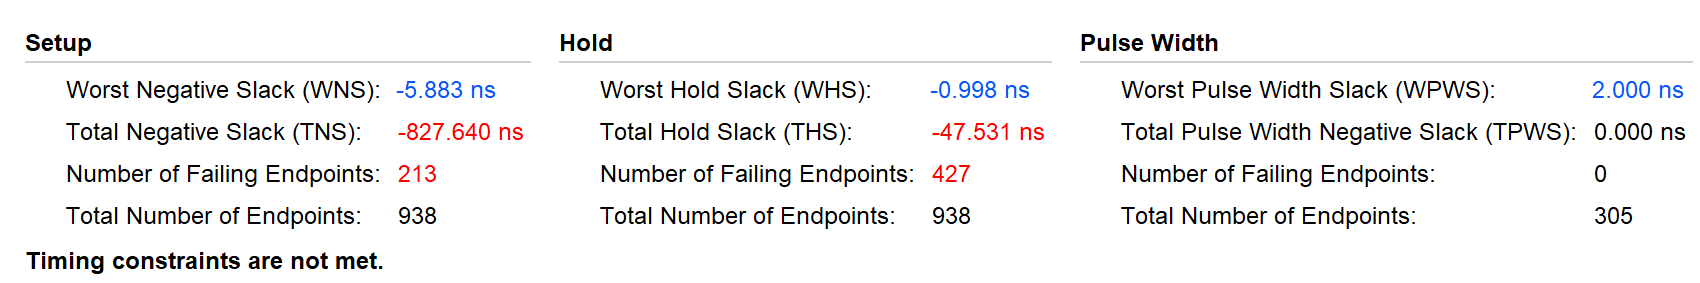
\includegraphics[width=\textwidth]{figures/time2.png}
  \caption{第二组实验的时序报告}
  \label{fig:time2}
\end{figure}

\begin{figure}[H]
  \centering
  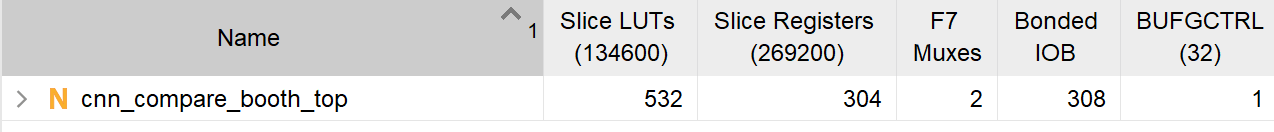
\includegraphics[width=\textwidth]{figures/util2.png}
  \caption{第二组实验的综合报告}
  \label{fig:util2}
\end{figure}

\begin{figure}[H]
  \centering
  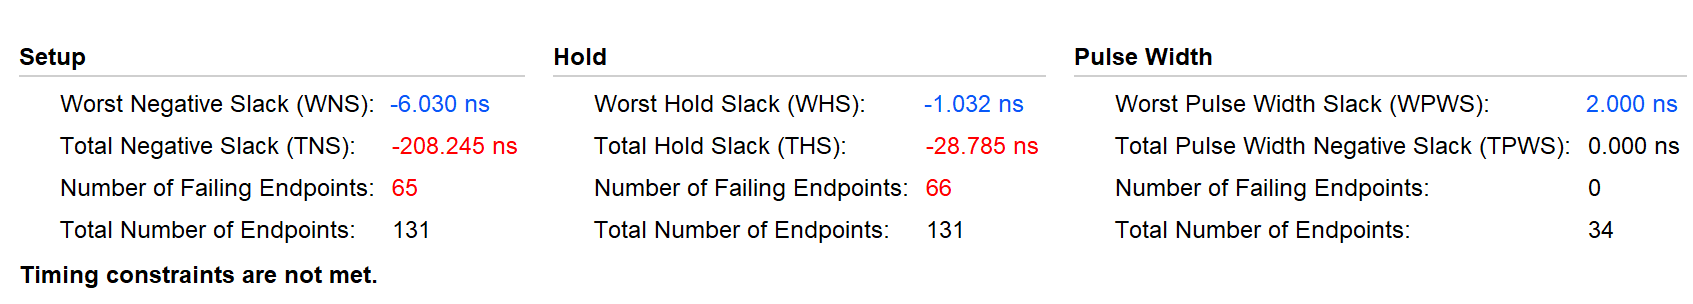
\includegraphics[width=\textwidth]{figures/time3.png}
  \caption{第三组实验的时序报告}
  \label{fig:time3}
\end{figure}

\begin{figure}[H]
  \centering
  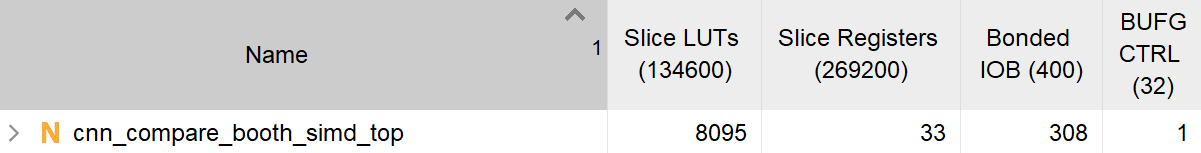
\includegraphics[width=\textwidth]{figures/util3.png}
  \caption{第三组实验的综合报告}
  \label{fig:util3}
\end{figure}


\begin{figure}[H]
  \centering
  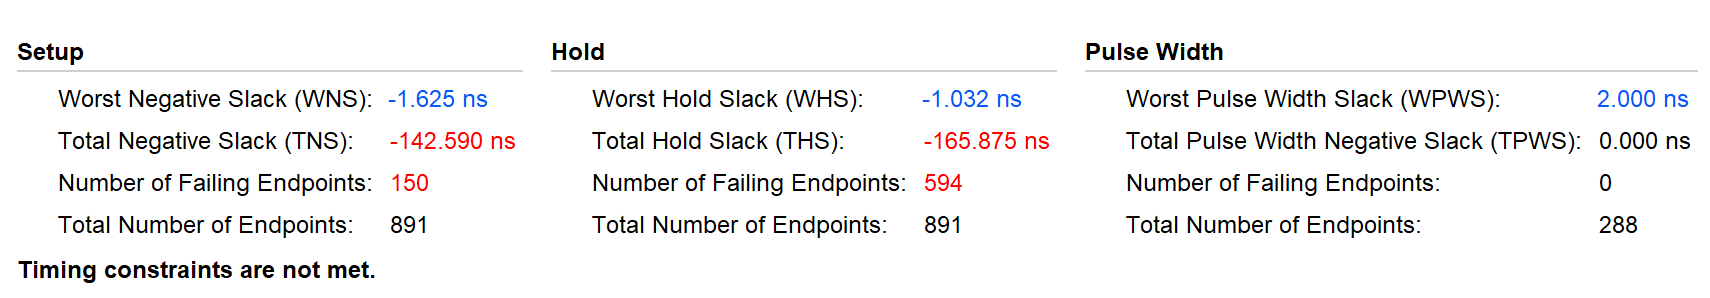
\includegraphics[width=\textwidth]{figures/time4.png}
  \caption{第四组实验的时序报告}
  \label{fig:time4}
\end{figure}

\begin{figure}[H]
  \centering
  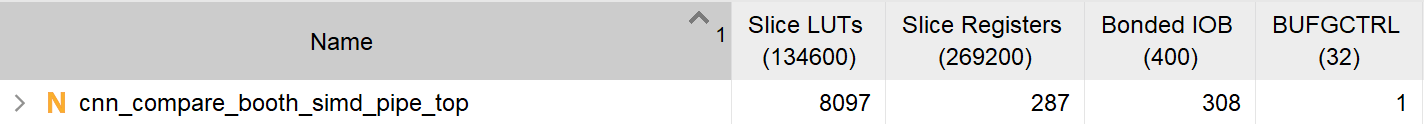
\includegraphics[width=\textwidth]{figures/util4.png}
  \caption{第四组实验的综合报告}
  \label{fig:util4}
\end{figure}

\subsection{第5组：在第4组基础上换用 DSP}
第 5 组仅作为第 4 组的 DSP 替换对照，不进入主四组主表。其比较结果如表 \ref{tab:dsp-compare} 所示。

\begin{table}[H]
\centering
\caption{第 4 组与第 5 组对比}
\label{tab:dsp-compare}
\begin{tabular}{lcc}
\toprule
指标 & 第 4 组：BoothWallace + SIMD + 流水线 & 第 5 组：DSP 替换版 \\
\midrule
LUT & 8097 & 1372 \\
FF & 287 & 287 \\
DSP & 0 & 81 \\
WNS/ns & -1.625 & -2.054 \\
估算$f_{\max}$/MHz & 150.94 & 141.76 \\
系统仿真周期数 & 3 & 3 \\
\bottomrule
\end{tabular}
\end{table}

这一组实验的结论比较明确：
\begin{itemize}
  \item 换用 DSP48E1 后，LUT 从 8097 大幅下降到 1372，逻辑资源减少约 83.1\%；
  \item 但在当前 200\,MHz 约束下，DSP 版的 WNS 并没有改善，反而从 -1.625\,ns 变为 -2.054\,ns；
  \item 功能与延迟周期保持不变，说明第 5 组达成了 ``只改实现、不改功能'' 的目标；
  \item 因此，对本工程当前 RTL 而言，DSP 替换带来的主要收益是逻辑资源迁移，而不是直接的性能提升。
\end{itemize}

\begin{figure}[H]
  \centering
  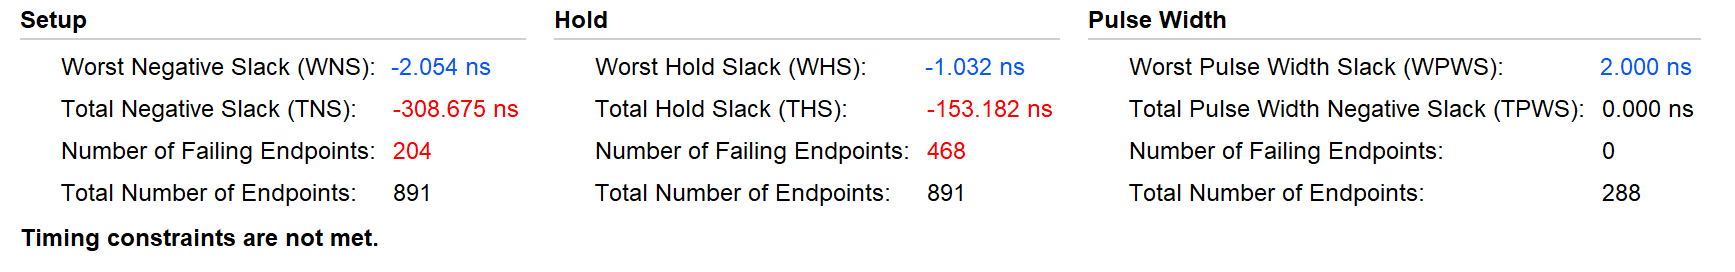
\includegraphics[width=\textwidth]{figures/time5.png}
  \caption{第五组实验的时序报告}
  \label{fig:time5}
\end{figure}

\begin{figure}[H]
  \centering
  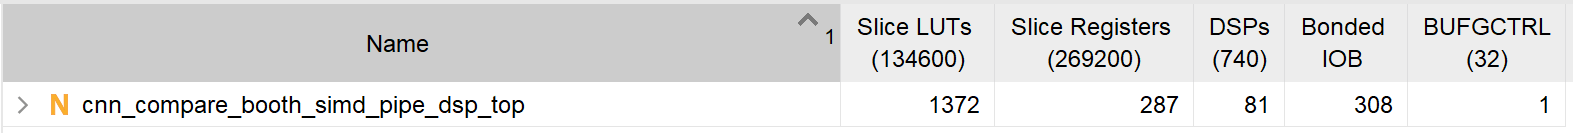
\includegraphics[width=\textwidth]{figures/util5.png}
  \caption{第五组实验的综合报告}
  \label{fig:util5}
\end{figure}

\subsection{优化版本系统仿真结果}
系统级仿真对 5 个顶层分别拉起 \texttt{start}，并显式检查输出与延迟行为。结果如表 \ref{tab:sim-system} 所示。

\begin{table}[H]
\centering
\caption{系统级仿真结果}
\label{tab:sim-system}
\begin{tabular}{lccc}
\toprule
实验组 & 输出结果 & 延迟周期 \\
\midrule
串行 &  \texttt{32'h9087635A} & 96 \\
串行 + BoothWallace &  \texttt{32'h9087635A} & 96 \\
BoothWallace + SIMD &  \texttt{32'h9087635A} & 1 \\
BoothWallace + SIMD + 流水线 &  \texttt{32'h9087635A} & 3 \\
DSP 替换版 &  \texttt{32'h9087635A} & 3 \\
\bottomrule
\end{tabular}
\end{table}

XSIM 日志中可以直接看到如下 PASS 信息：
\begin{verbatim}
CASE=1 PASS cycles=96 out=9087635a
CASE=2 PASS cycles=96 out=9087635a
CASE=3 PASS cycles=1  out=9087635a
CASE=4 PASS cycles=3  out=9087635a
CASE=5 PASS cycles=3  out=9087635a
ALL TESTS PASSED.
\end{verbatim}

图 \ref{fig:wave-pipe} 给出了第 4 组流水线版本的关键内部波形。可以看到 \texttt{vld\_pipe} 按 \texttt{001 $\rightarrow$ 010 $\rightarrow$ 100} 依次推进，卷积结果寄存、ReLU 结果寄存和池化输出寄存依次有效，最终在第 3 个周期输出 \texttt{0x9087635A}。

\begin{figure}[H]
  \centering
  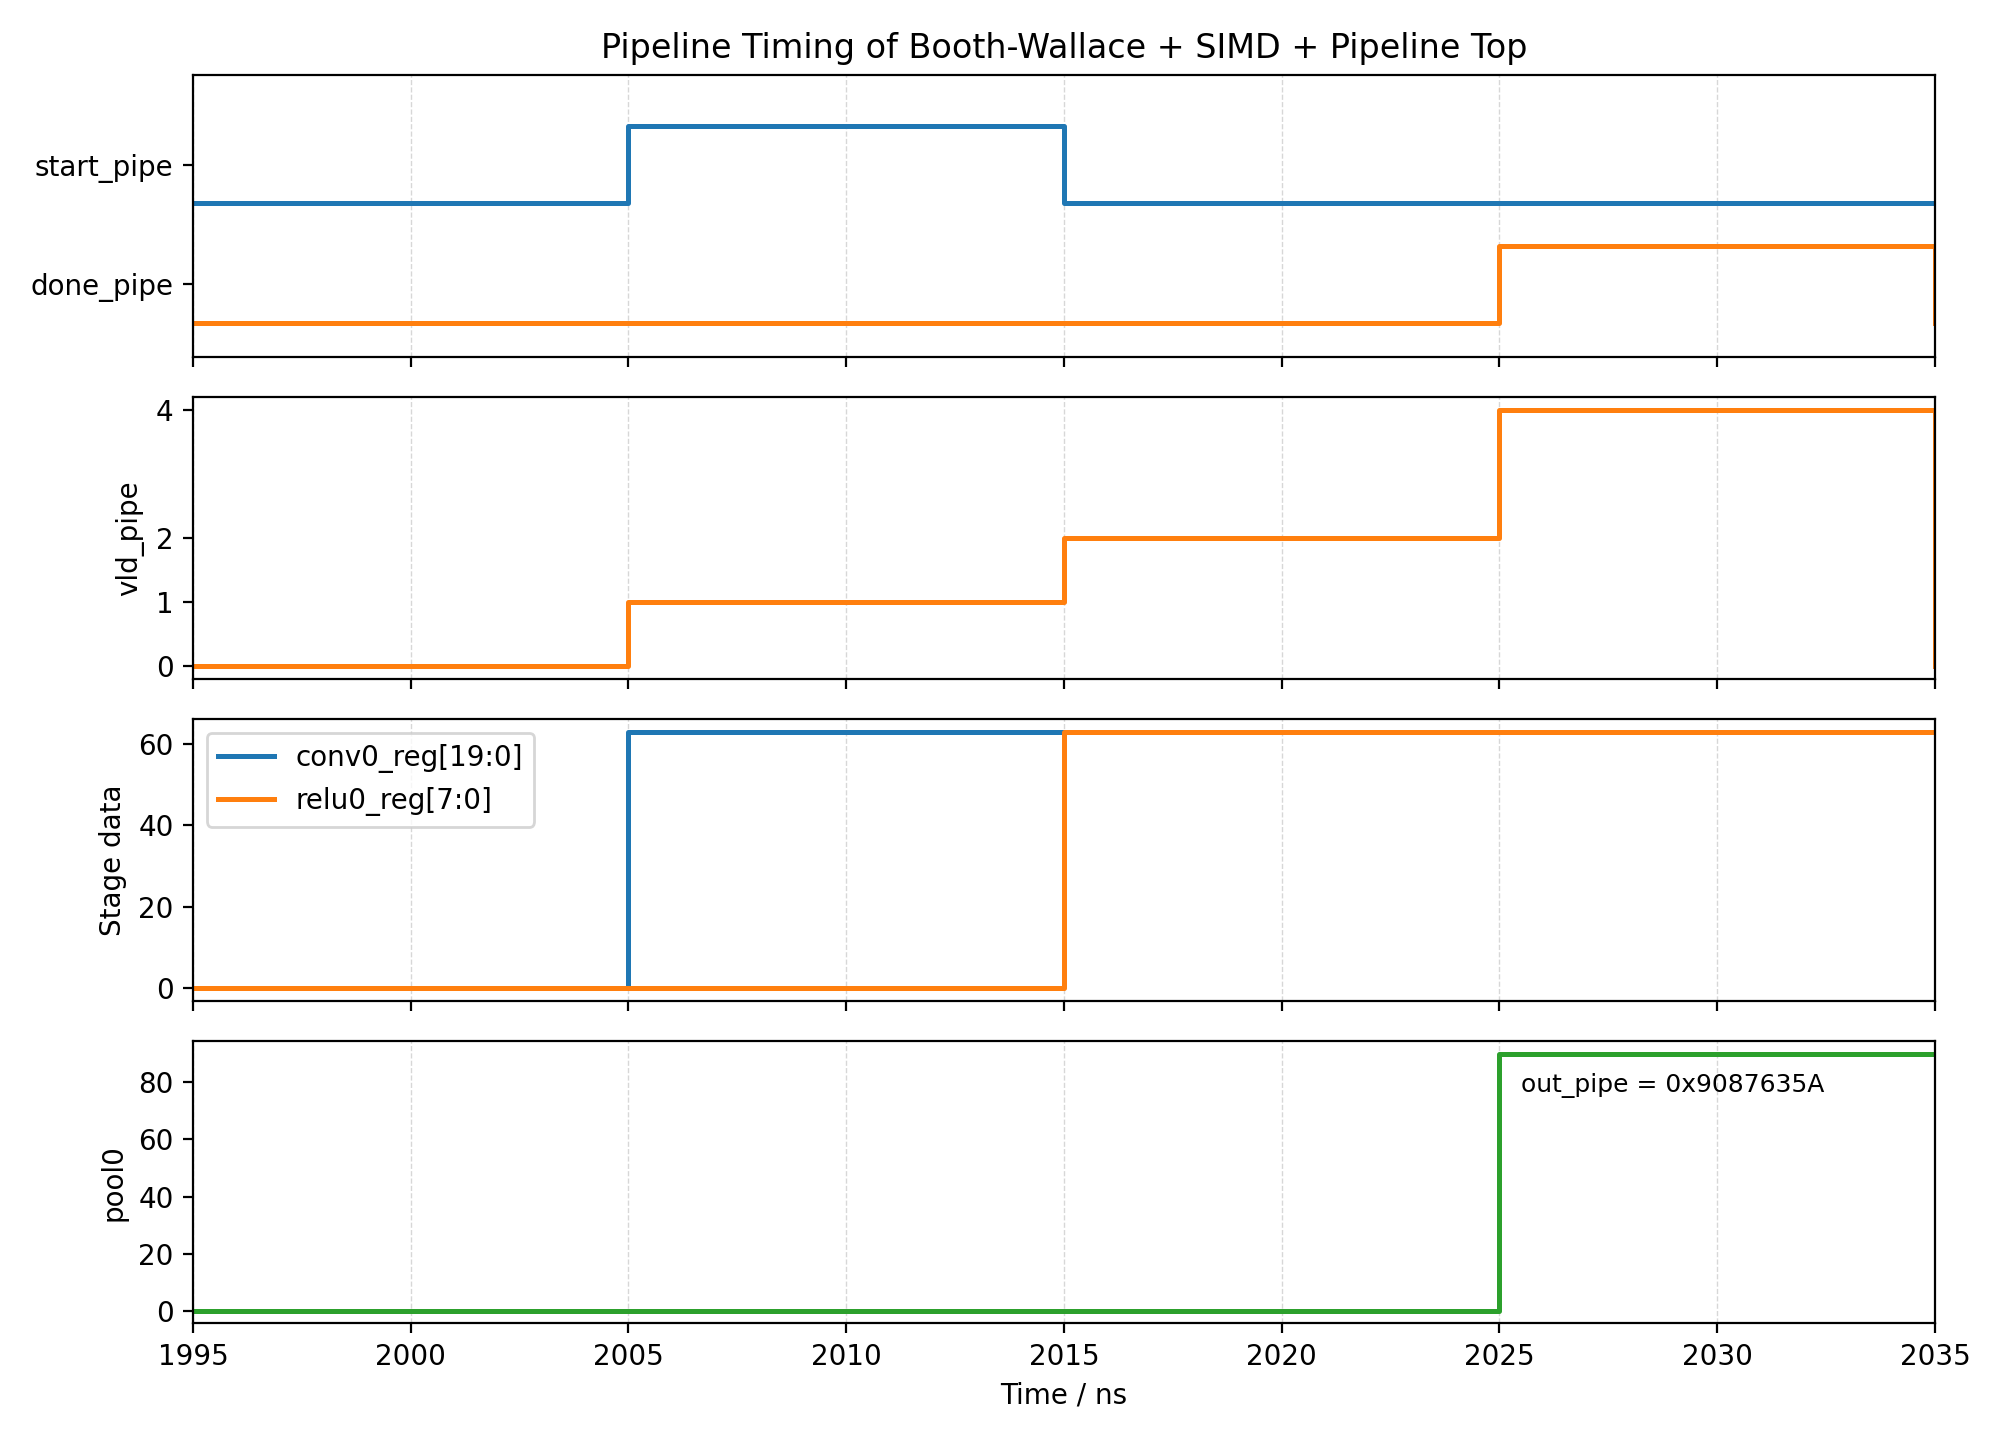
\includegraphics[width=\textwidth]{figures/wave_pipeline_timing.png}
  \caption{流水线波形：卷积寄存、ReLU 寄存与输出寄存的三级推进}
  \label{fig:wave-pipe}
\end{figure}

\section{实验收获}
\begin{itemize}
  \item 完整实现并验证了 8 位定点卷积、ReLU 激活和平均池化三段链路，对 CNN 基础算子在 FPGA 上的组织方式有了更具体的理解。
  \item 通过把 5 组实验拆成独立顶层，进一步体会到 ``便于综合分析的结构'' 与 ``便于功能复用的结构'' 并不总是同一件事。
  \item BoothWallace 乘法器、SIMD 路径和 3 级流水线都已经在工程中落地，并通过统一 testbench 验证了功能一致性。
  \item 从 Vivado 报告中可以看出，优化并不总会直接转化为更高主频；关键路径位置、寄存器边界和布线代价同样会改变最终结果。
  \item DSP 替换版说明了另一类典型工程取舍：它显著降低了 LUT 占用，但在当前结构下并未直接带来性能收益。
\end{itemize}

\section{附：源码目录}
\begin{itemize}
  \item \verb|project1/src/baseline/|：串行基线实现，包括 \verb|mul8.v|、\verb|add8.v|、\verb|relu_s20.v|、\verb|div4.v|、\verb|cnn_chain_core_base.v| 等；
  \item \verb|project1/src/optimized/|：BoothWallace、SIMD、流水线和 DSP 版本实现；
  \item \verb|project1/sim/|：模块级与系统级 testbench；
  \item \verb|project1/scripts/|：Vivado 批处理与波形导出脚本；
  \item \verb|project1/report/|：本报告与图片素材；
  \item \verb|project1/build/|：综合输出与仿真波形。
\end{itemize}

\end{document}